\RequirePackage{fix-cm} 

%% Definiere Klasse
\documentclass[11pt, a4paper,oneside]{scrbook} 	

%% misc
%\usepackage{cmbright}												% streifenlose computer modern fonts
\usepackage[T1]{fontenc}											% T1 fonts für gute pdf-Ausgabe
%\usepackage[ansinew]{inputenc}										% wegen deutschen Umlauten
\usepackage[automark]{scrpage2}										% Koma Headers

\usepackage[utf8]{inputenc}
\usepackage[english, ngerman]{babel}
% Wechseln durch \begin{otherlanguage}{english}.. \end{otherlanguage}


% \usepackage{boxit}	 												% frame handling
\usepackage{nag}													% warn user on outdated packages
\usepackage[linktocpage]{hyperref}									% links in pdf, thumbnails
\usepackage{soul}													% emphasizing text, underlining				
\usepackage[onehalfspacing]{setspace}								% 1.5, change line spaces by \singlespacing \doublespacing


%% Tabellen
\usepackage{multicol} 												% Mehrfache Zeilen / Spalten
\usepackage{multirow}												% Mehrfache Zeilen in Tabellen
\usepackage[margin=10pt,labelfont=bf]{caption}						% Tabellen-Kopf
\usepackage{hhline}													% horizontale Linien
\usepackage{longtable}												% über Seitenumbruch hinauslaufende Tabelle
\usepackage{booktabs}												% dicke Tabellenlinien \toprule
\usepackage{tabularx}												

%% math, symbols
\usepackage{amsmath}												% AMS Math like brackets, integrals...
\usepackage{fixmath}												% big greek letters italic in math mode
\usepackage{array}													% matrices
\usepackage{units}		  											% includes nicefrac, nicer fracs for one line, SI-Units
\usepackage{trfsigns}												% symbole für transformationen
\usepackage{textcomp}												% einfache Sonderzeichen, z.B. \texteuro
\usepackage{gensymb}												% correct greek letters in units,\micro instead of \mu
\usepackage[integrals]{wasysym}										% for integrals like \oiint
\usepackage{ziffer}													% let"',"' be a valid delimiter in formulaes
\usepackage{dsfont}													% für andere Mengenzeichen, $\mathds{ABCDEFGHIJKLMNOPQRSTUVWXYZ}$


%% graphics
%\usepackage[activate]{pdfcprot}									% use margin kerning (character protruding) (Opt. Randausgleich)
\usepackage{microtype}												% character protruding, font expansion - instead of pdfcprot
\usepackage{graphicx}												% include graphics
\usepackage{wrapfig} 												% graphics in text
\usepackage{floatflt}												% graphics/tables in text
\usepackage{rotating} 												% rotating elements
\usepackage{listings}												% for programming source code
\usepackage[svgnames]{xcolor}										% colors for listings
\usepackage{psfrag}													% Text in .eps Grafiken ersetzen

%% Definiere Layout
\usepackage[top=2.5cm,left=3.5cm,right=2.5cm,bottom=3cm]{geometry}

%%%%%%%%%%%%%%%%%%%%%%%%%%%%%%%%%%%%%%%%%%%%%%%%%%%%%%%%%%%%%%%%%%%

% Allgemeine Definitionen des Dokumentes
% Allgemeine Schalter-Änderung von Standardeinstellungen
\frenchspacing

% keine längeren Leerzeichen nach Satzende/Abkürzungen mit Punkt
\setlength{\parindent}{0pt}

% kein Einzug bei neuem Absatz
\setlength{\parskip}{1.5ex plus0.5ex minus 0.5ex}

% Wortabstände optimal einstellen  Verhindern von herausragenden Zeilen
\tolerance 1414
\hbadness 1414
\emergencystretch 1.5em
\hfuzz 0.3pt
\widowpenalty=10000
\vfuzz \hfuzz
\raggedbottom
\brokenpenalty=10000

% Trennung bei Seitenumbruch
\setlength{\headheight}{1cm}

% Höhe der Kopfzeile
\addtolength{\footnotesep}{2pt}									


% Setze Überschriftentiefe
\setcounter{secnumdepth}{3}										

% Nummerierung der Kapitel
\setcounter{figure}{4}															
% Bilder
\setcounter{tocdepth}{3}														

% Einstellungen für Kopf- und Fußzeilen
\pagestyle{scrheadings}       % nutze scrheader
\clearscrheadings             % lösche alle vorhandenen header

%\addtokomafont{pagehead}{\normalsize\upshape}  % nichtkursive Kopf-/Fußzeilen
\setheadsepline{.05pt}					% trennlinie oben
\setfootsepline{.05pt}					% trennlinie unten


\automark[section]{chapter}   % links chapter, rechts section

% variere nach ein-/zweiseitig
\makeatletter
\if@twoside											% bei zweiseitig
	\lehead{\leftmark}            % setze Kapitel linke Seite oben
	\rohead{\rightmark}           % setze Abschnitt rechte Seite oben
	\lefoot{\pagemark}            % Seitennummer unten links
	\rofoot{\pagemark}            % Seitennummer unten rechts
	\lofoot{\Autor}       				% Name des Verfassers nur linke Seite
\else														% einseitig
	\ihead{\leftmark}            	% setze linke kopfzeile
	\ohead{\rightmark}           	% setze rechte kopfzeile
	\ofoot{\pagemark}             % seitennummer unten rechts
	\ifoot{\Autor}       					% Name des Verfassers unten links
\fi

% Bei Kapiteln ohne Subsection wird Kapitelname eingeblendet, nutze
% \markright{}, um den \rohead freizulassen

\makeatother         								

% "input" ersetzt den Text, "include" erstellt neue Seite

%%%%%%%%%%%%%%%%%%%%%%%%%%%%%%%%%%%%%%%%%%%%%%%%%%%%%%%%%%%%%%%%%%%%

% Benutzer Definitionen
%%%%%%%%%%%%%%%%%%%%%%%%%%%%%%%%%%%%%%%%%%%%%%%%%%%%

% Autor, Titel, Datum der These
\newcommand*{\Title}{Erstellung eines Plugin unter Verwendung der Entwicklungsumgebung Unity zur Implementierung des "Motion-Tracked Binaural"-Verfahrens}
\newcommand*{\Autor}{Maximilian Lehmer}
\newcommand*{\Datum}{Berlin, September 2018}
\title{\Title}
\author{\Autor} 
\date{\Datum}

% Beispiel für Definition neuer Kommandos für häufig gebrauchte Konstrukte

\newcommand{\tfk}[1]{\textsl{\texttt{#1}}}
\newcommand{\fett}[1]{\textbf{#1}}
\newcommand{\kursiv}[1]{\textit{#1}}
\newcommand{\pbb}{\parbox}
\newcommand{\sst}{\scriptstyle}

										
   										

%%%%%%%%%%%%%%%%%%%%%%%%%% START %%%%%%%%%%%%%%%%%%%%%%%%%%%%%%%%%%%

\begin{document}

    % Titelblatt
	%\thispagestyle{empty}
\begin{titlepage} 
\begin{centering}

	% Header
	\begin{figure}[!h]
		% TU Logo
  	\begin{minipage}{0.4\linewidth}
			\begin{center}
				\includegraphics[scale=1]{Titelblatt/tu-logo.eps} 
  		\end{center}  
  	\end{minipage}
		\hfill
		% EMSP Logo
  	\begin{minipage}{0.45\linewidth} 
  		\begin{center}
				\includegraphics[scale=0.3]{Titelblatt/Logo_final.eps} 
  		\end{center}    
  	\end{minipage}
	\end{figure}
	
	% vertikaler Zwischenraum
	\vspace{20mm}
	
	% Titel der Arbeit
	\LARGE

	Bachelorarbeit
	
	\textbf{\Title}\\[2cm]

	
	\large
	erstellt von\\
	
	% Name des Verfassers
	\Autor\\
	Matrikel: 339664\\[25mm]

	% Betreuer
	\begin{minipage}{\linewidth} 
		\begin{tabbing}
    	Erstprüfer:\quad \= Prof. Dr.-Ing. R. Orglmeister, FG EMSP\\
    	Zweitprüfer:             \> Prof. Dr. S. Weinzierl, FG Audiokommunikation\\
    	Betreuer:             \> D. Ackermann, FG Audiokommunikation \\
    			
  	\end{tabbing}
  \end{minipage}
	
	% vertikaler Zwischenraum
	\vspace{10mm}
	
	\normalsize
	{Technische Universität Berlin}\\ {Fakultät IV}\\ {Institut für Energie- und Automatisierungstechnik}\\ {Fachgebiet Elektronik und medizinische Signalverarbeitung}\\
	\Datum\\
\end{centering}
\end{titlepage}
	
	
	% Leere Seite
	\newpage 
    \thispagestyle{empty}
    \quad 
    \newpage
    
    % Einbinden aller Literatureinträge
    \nocite{*}														
    
%%%%%%%%%%%%%%%%%%%%%% VORSPANN %%%%%%%%%%%%%%%%%%%%%%%%%%%%%%%%%%%%
    
    % römische Seitennummerierung
	\pagenumbering{roman}											
	
	% Kurzfassung				
	\chapter*{Kurzfassung}
\addcontentsline{toc}{chapter}{Kurzfassung}

Hier steht eine Kurzfassung der Arbeit. Im Englischen wird für dieses Kapitel auch die Überschrift ``abstract'' verwendet.

Der Unterschied zur ``Einleitung'' besteht darin, dass hier nicht der Aufbau der Arbeit, d.\,h.\ die
einzelnen Kapitel vorgestellt werden, sondern nur die bearbeitete Aufgabe und
Vorgehensweise kurz beschrieben und eine Zusammenfassung der Ergebnisse gegeben wird. Daher sollte
die ``Kurzfassung'' nicht länger als eine halbe Seite sein.
								
	% Abkürzungen
	%Abkürzungsverzeichnis
\chapter*{Abkürzungen und Bezeichnungen}
\addcontentsline{toc}{chapter}{Abkürzungen und Bezeichnungen}

\thispagestyle{empty}													% ohne Kopf und Fußzeilen

% setzen des Tabs
\begin{tabbing}
-------------------\=--------------------------------\kill

% Abkürzungen

MTB     \>Motion-Tracked Binaural\\
ITD     \>interaurale Zeitdifferenz (engl. interaural time difference)\\
ILD     \>interaurale Pegeldifferenz (engl. interaural level difference)\\
FFT     \>Fast Fourier Transform\\
STFT    \>Short Time Fourier Transform\\
\\
AES     \>Audio Engineering Society\\



\end{tabbing}

\rule{10cm}{.3mm}
% Bezeichnungen

\begin{tabbing}
-------------------\=--------------------------------\kill

$P(A)$      \>Wahrscheinlichkeit für Ereignis A\\
$G$         \>Graph\\
$\mu$       \>Mittelwert\\

\end{tabbing}
								
	% Erklärung
	% Erklärung
\thispagestyle{empty}													% ohne Kopf und Fußzeilen
\begin{LARGE}
	\textbf{Erklärung}
\end{LARGE}

\vspace{1cm}

Die selbständige und eigenständige Anfertigung versichert an Eides statt.
\vspace{2cm}

Berlin, den \today

\vspace{1cm}
%\rule{_Breite_}{_Stärke_}		% anders herum ist's vertikal

\rule{0.3\textwidth}{0.4pt}

Unterschrift

%\Datum
\vspace*{6cm}



	
	% Danksagung (optional)
	% Danksagung

\begin{LARGE}
    \textbf{Danksagung}
\end{LARGE}

\vspace{1cm}

Der Autor dankt hiermit allen, die durch ihre Unterstützung zur
Entstehung dieser Arbeit beigetragen haben. Besonderer Dank gilt
vor allen Dingen den Betreuern seitens der Dingsbums AG, den
Damen und Herren Dr. Sowieso etc.

\newpage
									
%%%%%%%%%%%%%%%%%%%%% INHALTSVERZEICHNIS %%%%%%%%%%%%%%%%%%%%%%%%%%%
	% Inhaltsverzeichnis
	\tableofcontents 
	
	% Leere Seite
	\newpage 
    \thispagestyle{empty}
    \quad 
    \newpage
    
%%%%%%%%%%%%%%%%%%% HAUPTTEIL %%%%%%%%%%%%%%%%%%%%%%%%%%%%%%%%%%%%%%
	
	\pagenumbering{arabic}
			
	\chapter[Einleitung]{Einleitung} 
\label{chap:Einl}						
	\chapter[Theoretische Grundlagen]{Theoretische Grundlagen} \label{chap:2_THEO}

\section{Grundlagen der akustischen Wahrnehmung}
\label{sec:2_GDAW}
    
    Hier wird ein kurzer Einleitungstext zu den Grundlagen der akustischen Wahrnehmung stehen.
    
    \subsection{Interaurale Zeitdifferenz}
    \label{subsec:2_ITD}
        
        Hier wird genauer auf die ITD eingegangen.
    
    \subsection{Interaurale Pegeldifferenz}
    \label{subsec:2_ILD}
    
        Und folglich hier nöher auf die ILD.

    
\section{Interpolationsverfahren}
\label{sec:2_IV}

Allgemeines zur Notwendigkeit der Interpolation.

    \subsection{Allgemeine Übersicht}
    \label{subsec:2_AUE}

    Hier erscheint eine Übersicht der "{}einfachen"{}  Interpolationsalgorithmen. Danach wird genauer auf die Interpolation im Frequenzbereich eingegangen.
    
    \subsection{Interpolation im Frequenzbereich}
    \label{subsec:ILD}

    
        \begin{enumerate}
            \item Blockschaltbild
            \item Mathematische Grundlagen
            \begin{enumerate}
                \item Fast Fourier Transform
                \item Short Time Fourier Transform
                \item Berechnung des Distanzkoeffizienten
            \end{enumerate}    
        \end{enumerate}

\section{Headtracking}
\label{sec:2_HT}

Hier wird die die Notwendigkeit des Headtrackings erläutert und zudem auf verschiedene Realisierungsmöglichkeiten eingegangen.
	\chapter[Stand der Forschung]{Stand der Forschung} 
\label{chap:SDF}
	\chapter[Implementierung des Plugin]{Implementierung des Plugin} \label{chap:Impl}
	\chapter[Evaluation]{Evaluation} 
\label{chap:Eval}


Als Bild (aus Word):
\begin{figure}[!htbp]
			\begin{center}
				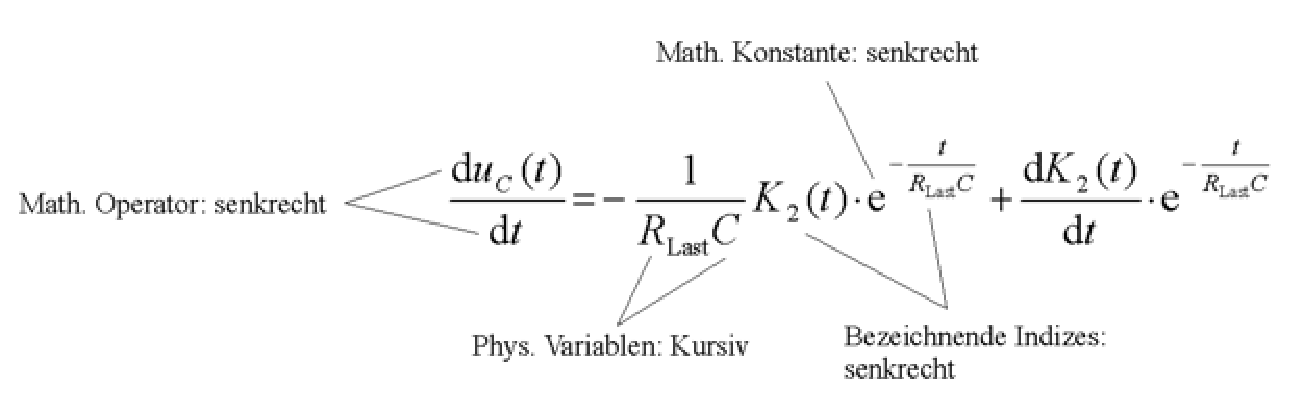
\includegraphics[scale=0.6]{5_Evaluation/formelbeispiel.eps}
				\caption{Formelbeispiel}
				\label{chap2:formelbeispiel}
  		\end{center}
\end{figure}


\begin{table}[!ht]
\caption[In Matlab]{Matlab-Befehle}
\label{tab:ML1}
\begin{tabular}{|| p{7cm} | p{6cm} ||} \hline\hline
I=eye(N);      																									& Einheitsmatrix \\ \hline
e=zeros(N,1); e(j)=1; 																					& Einheitsvektor\\ \hline
D=diag([d11,d22,...,dNN]); 																			& Diagonalmatrix \\ \hline
J=rot90(eye(N)); 																								& Koidentitätsmatrix \\ \hline
E=ones(M,N); 																										& Einsmatrix \\ \hline
eins=ones(N,1); 																								& Einsvektor \\ \hline
t1=[t11,t12,...,t1N]; t2=[t11,t21,...,tN1]; 										& \\
T=toeplitz(t1,t2);  																						& Toeplitzmatrix \\ \hline
t=[t11,t12,...,t1N]; T=toeplitz(t); 														& symmetrische Toeplitzmatrix \\ \hline
x=[x1,x2,...,xN]; v=rot90(vander(x))'; 													& Vandermonde-Matrix \\ \hline
L=tril(A); 																											& untere Dreiecksmatrix der Matrix A \\ \hline
U=triu(A); 																											& obere Dreiecksmatrix der Matrix A \\ \hline\hline
\end{tabular}
\end{table}
	\chapter[Fazit und Ausblick]{Fazit und Ausblick} 
\label{chap:Fazit}

Ich fahr zitternd nach Hause und genieße den Ausblick.

%%%%%%%%%%%%%%%%% ANHANG %%%%%%%%%%%%%%%%%%%%%%%%%%%%%%%%%%%%%%%%%%%

\begin{appendix}
		% Anhang A - Quellcode

\chapter[Erstellter Programmcode]{Erstellter Programmcode}
%
Für das Einfügen erstellten Programmcodes bietet sich das Paket \textsl{listings} an. Der Funktionsumfang des Paketes ist sehr groß, weshalb hier nur ein Beispiel gezeigt werden soll, dass mit den folgenden Einstellungen erzeugt wurde:
{\lstset{language=[LaTeX]{TeX}, basicstyle=\small, keywordstyle=\color{DarkBlue}}
\begin{lstlisting}
\lstset{language=Matlab, basicstyle=\small, xleftmargin=15pt,
        keywordstyle=\color{DarkBlue}, numbers=left, 
        numberstyle=\tiny, commentstyle=\color{DarkGreen}}.
\end{lstlisting}}
%
Für weitere Informationen zu Mölichkeiten des Pakets sei auf dessen Dokumentation verwiesen.
\section{Matlab-Code}
% set style for matlab listings
\lstset{language=Matlab, basicstyle=\small, xleftmargin=15pt,
				keywordstyle=\color{DarkBlue}, numbers=left, 
				numberstyle=\tiny, commentstyle=\color{DarkGreen}}
%
Der folgende Code dient zur Erzeugung des Bildes . Die Einrückungen im Quelltext sollen lediglich die Möglichkeiten des listings-Paket zeigen.

\begin{lstlisting}
%----------------------------------------------
% Make an image that uses only 8 levels/colors.
%----------------------------------------------
imagesc(floor(8*rand(20)))

%-----------------------------------------------------------
% Make an 8-row color map from the original 64-row colormap.
%-----------------------------------------------------------
	m64 = colormap; % Beispiel Einrung
m8=m64(1:8:end,:);
	colormap(m8);   % Beispiel Einrung

%---------------------
% Label new color map.
%---------------------
h = colorbar % Make colorbar and save handle.
set(h, 'ytick', (1:2:16)*7/16) % Assign positions of ticks
labels = strvcat('zero','one','two','three','four', ...
'five','six','seven'); %
%Make  levels for ticks.
set(h, 'yticklabel', labels) % Assign tick labels.
\end{lstlisting}


		% Anhang B - Quick Start Guide

\chapter[Quick Start Guide]{Quick Start Guide}


		% Anhang C - Unknown

\chapter[Unknown]{Unknown}

	\end{appendix}

%%%%%%%%%%%%%%%%% ABBILDUNGSVERZEICHNIS %%%%%%%%%%%%%%%%%%%%%%%%%%%%%

	\listoffigures
	\addcontentsline{toc}{chapter}{Abbildungsverzeichnis}
	
%%%%%%%%%%%%%%%%% TABELLENVERZEICHNIS %%%%%%%%%%%%%%%%%%%%%%%%%%%%%%%

	\listoftables
	\addcontentsline{toc}{chapter}{Tabellenverzeichnis}

%%%%%%%%%%%%%%%%% LITERATURVERZEICHNIS %%%%%%%%%%%%%%%%%%%%%%%%%%%%%%
	
	\raggedright													% Literatur im Flattersatz (v.a. wegen URLs)
	\bibliography{Literatur/Literatur}
	\bibliographystyle{alphadin}
	\addcontentsline{toc}{chapter}{Literaturverzeichnis}

\end{document}
